%%%
% Plantilla de Memoria
% Modificación de una plantilla de Latex de Nicolas Diaz para adaptarla 
% al castellano y a las necesidades de escribir informática y matemáticas.
%
% Editada por: Mario Román
%
% License:
% CC BY-NC-SA 3.0 (http://creativecommons.org/licenses/by-nc-sa/3.0/)
%%%

%%%%%%%%%%%%%%%%%%%%%%%%%%%%%%%%%%%%%%%%%
% Thin Sectioned Essay
% LaTeX Template
% Version 1.0 (3/8/13)
%
% This template has been downloaded from:
% http://www.LaTeXTemplates.com
%
% Original Author:
% Nicolas Diaz (nsdiaz@uc.cl) with extensive modifications by:
% Vel (vel@latextemplates.com)
%
% License:
% CC BY-NC-SA 3.0 (http://creativecommons.org/licenses/by-nc-sa/3.0/)
%
%%%%%%%%%%%%%%%%%%%%%%%%%%%%%%%%%%%%%%%%%

%----------------------------------------------------------------------------------------
%	PAQUETES Y CONFIGURACIÓN DEL DOCUMENTO
%----------------------------------------------------------------------------------------

%%% Configuración del papel.
% microtype: Tipografía.
% mathpazo: Usa la fuente Palatino.
\documentclass[a4paper, 11pt]{article}
\usepackage[protrusion=false,expansion=false]{microtype}
\usepackage{mathpazo}
\usepackage[section]{placeins}

% Indentación de párrafos para Palatino
\setlength{\parindent}{0pt}
  \parskip=8pt
\linespread{1.05} % Change line spacing here, Palatino benefits from a slight increase by default


%%% Castellano.
% noquoting: Permite uso de comillas no españolas.
% lcroman: Permite la enumeración con numerales romanos en minúscula.
% fontenc: Usa la fuente completa para que pueda copiarse correctamente del pdf.
\usepackage[spanish,es-noquoting,es-lcroman]{babel}
\usepackage[utf8]{inputenc}
\usepackage[T1]{fontenc}
\selectlanguage{spanish}


%%% Gráficos
\usepackage{graphicx} % Required for including pictures
\usepackage{wrapfig} % Allows in-line images
\usepackage[usenames,dvipsnames]{color} % Coloring code


%%% Matemáticas
\usepackage{amsmath}
\usepackage{amsthm} 

%%% Bibliografía
\makeatletter
\renewcommand\@biblabel[1]{\textbf{#1.}} % Change the square brackets for each bibliography item from '[1]' to '1.'
\renewcommand{\@listI}{\itemsep=0pt} % Reduce the space between items in the itemize and enumerate environments and the bibliography

%----------------------------------------------------------------------------------------
%	ENTORNO EJERCICIOS
%----------------------------------------------------------------------------------------
\newtheoremstyle{}
  {\topsep}   % ABOVESPACE
  {\topsep}   % BELOWSPACE
  {\itshape}  % BODYFONT
  {0pt}       % INDENT (empty value is the same as 0pt)
  {\bfseries} % HEADFONT
  {.}         % HEADPUNCT
  {\newline} % HEADSPACE
  {}          % CUSTOM-HEAD-SPEC


\theoremstyle{plain}
\newtheorem{nej}{Ejercicio}[section]

%----------------------------------------------------------------------------------------
%	TÍTULO
%----------------------------------------------------------------------------------------
% Configuraciones para el título.
% El título no debe editarse aquí.
\renewcommand{\maketitle}{
  \begin{flushright} % Right align
  
  {\LARGE\@title} % Increase the font size of the title
  
  \vspace{50pt} % Some vertical space between the title and author name
  
  {\large\@author} % Author name
  \\\@date % Date
  \vspace{40pt} % Some vertical space between the author block and abstract
  \end{flushright}
}

%% Título
\title{\textbf{Fundamentos de Redes}\\ % Title
Definición e implementación de un protocolo de aplicación} % Subtitle

\author{\textsc{Sofía Almeida Bruno\\Fernando de la Hoz Moreno} % Author
\\{\textit{Universidad de Granada}}} % Institution

\date{\today} % Date



%----------------------------------------------------------------------------------------
%	DOCUMENTO
%----------------------------------------------------------------------------------------

\begin{document}

\maketitle % Print the title section
\section{Descripción de la aplicación}
Nuestro proyecto se basa en la realización de una calculadora con diferentes funcionalidades, diseñada según en el paradigma cliente-servidor.
Los clientes son los usuarios que solicitarán el procesamiento de un cálculo (operaciones simples o resolución de una ecuación) y el servidor será la calculadora que se encargará de atender las peticiones de los clientes y darles respuesta.
Para ello, utilizaremos los sockets TCP que nos garantizan que la información que se intercambia entre los usuarios y la calculadora es fiable, la sobrecarga del TCP sobre el UDP no nos afecta.

\section{Diagrama de estados del servidor}
	\begin{figure}[!h]
		\centering
		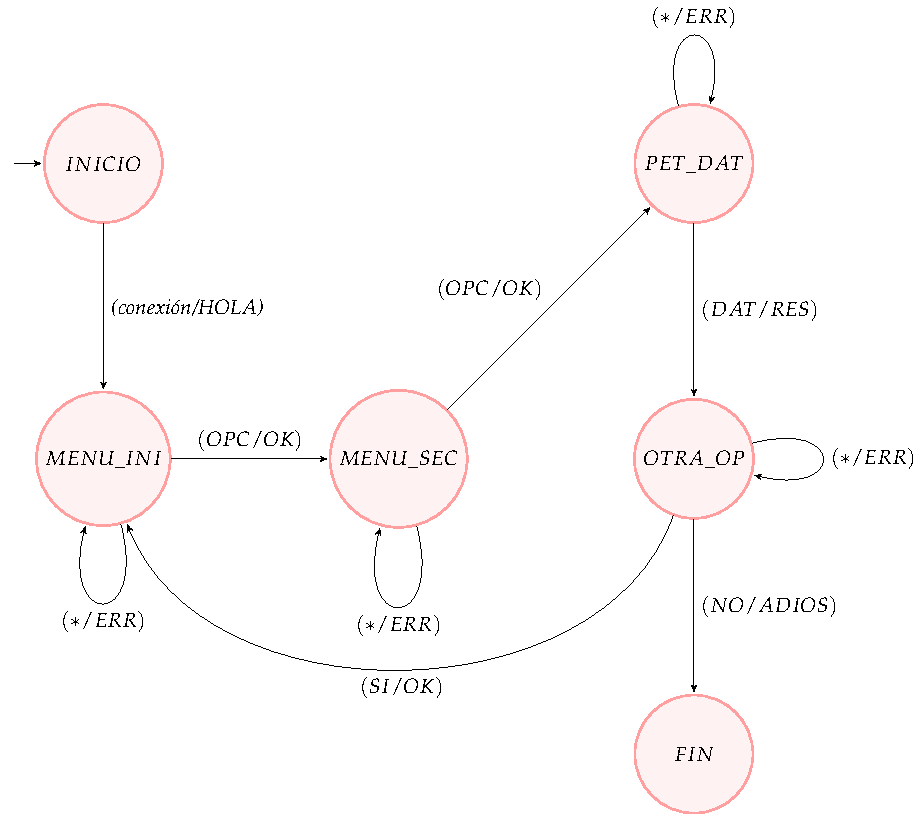
\includegraphics[scale=0.7]{./diagrama}
	\end{figure}

Partiendo de un estado $INICIO$, cuando el cliente establece la conexión llegamos a un menú inicial ($MENU\_INI$) donde el usuario puede elegir si quiere realizar una operación simple o resolver una ecuación. Esta elección lo llevará a un menú secundario ($MENU_SEC$), específico según la opción, donde a su vez tendrá que decidir la operación concreta o el grado de la operación a resolver. Pasará entonces a un estado de petición de datos ($PET_DAT$) donde indicará los datos con los que operar, el servidor responderá mandando el resultado de la operación y llegará a otro estado ($OTRA_OP$) donde el cliente puede elegir si quiere realizar otra operación o finalizar la ejecución ($FIN$). 
\section{Mensajes que intervienen}

\begin{table}[]
\centering
\label{my-label}
\begin{tabular}{lll}
\hline
\multicolumn{1}{|l|}{Código} & \multicolumn{1}{l|}{Cuerpo} & \multicolumn{1}{l|}{Descripción}   \\ \hline
001                          & HOLA                        & Confirmación de conexión realizada \\
002                          & OPC                         & Opción elegida                     \\
003                          & OK                          & Elección verificada                \\
004                          & ERR                         & Opción incorrecta                  \\
005                          & DAT                         & Datos con los que operar           \\
006                          & RES                         & Resultado de la operación          \\
007                          & SI                          & Realizar otra operación            \\
008                          & NO                          & No realizar otra operación         \\
009                          & ADIOS                       & Finalización de la conexión       
\end{tabular}
\end{table}

\section{Evaluación de la aplicación}
% Añadir capturas de la ejecución y explicarlas
\end{document}